\documentclass{article} % For LaTeX2e
\usepackage{nips13submit_e,times}
\usepackage{hyperref}
\usepackage{url}
\usepackage{graphicx}
\usepackage{amsfonts}
\usepackage{enumitem}
\usepackage{xparse}




\title{2D visualization of high-dimensional cellular protein data for cancer detection}


\author{
Amit Badlani \\
Dept. of Electrical Engineering Stanford University \\
\texttt{abadlani@stanford.edu} \\
\AND
Andre Esteva \\
Dept. of Electrical Engineering Stanford University \\
\texttt{andre.esteva@gmail.com} \\
\And
Anand Sampat\\
Dept. of Electrical Engineering Stanford University \\
\texttt{asampat@stanford.edu} \\
}

% The \author macro works with any number of authors. There are two commands
% used to separate the names and addresses of multiple authors: \And and \AND.
%
% Using \And between authors leaves it to \LaTeX{} to determine where to break
% the lines. Using \AND forces a linebreak at that point. So, if \LaTeX{}
% puts 3 of 4 authors names on the first line, and the last on the second
% line, try using \AND instead of \And before the third author name.

\newcommand{\fix}{\marginpar{FIX}}
\newcommand{\new}{\marginpar{NEW}}

\nipsfinalcopy % Uncomment for camera-ready version

\DeclareDocumentEnvironment{steps}%
{O{Step}}% If no argument is given the label defaults to 'Step'
{\begin{enumerate}[label=#1 \arabic*]}%
{\end{enumerate}}

\makeatletter% http://tex.stackexchange.com/questions/29517/forcing-new-line-after-item-number-in-enumerate-environment/29518#29518
\def\step{%
   \@ifnextchar[ \@step{\@noitemargtrue\@step[\@itemlabel]}}
\def\@step[#1]{\item[#1]\mbox{}\\\hspace*{\dimexpr-\labelwidth-\labelsep}}
\makeatother

\begin{document}


\maketitle

\begin{abstract}

\end{abstract}

\section{Introduction and Problem Statement}
\label{intro}
In the field of cancer immunology, scientists use the protein content of immune system cells as a way to identify a cell�s corresponding type. For example, immune system cells, which are contained in bone marrow, are comprised of a variety of cell types, and to a large degree, each type is uniquely identifiable by both intracellular proteins (IP) and surface proteins (SP). Highly sophisticated methods have been developed that process cells and return information on the types and quantities of proteins expressed in those cells. This data can then be viewed by an expert in the field and categorized. The laborious process of viewing the different dimensions of protein expression and categorizing a cell is known as gating. 

Is there order to this data? Does cell type, as a function of protein expression, have some structure in multi-dimensional protein space which can be understood and segmented? Can this data be mapped onto a different multi-dimensional space (MDS) where structure is better defined? These are questions of interest to cancer immunologists. If a well-defined structure exists which separates healthy immune system cells from other types of cells, such structure could be leveraged to identify cancer cells.

Cells evolve. Stem cells become progenitor cells, which become monocytes, etc. As they change, so do the types and quantities of proteins that they express. This leads to a shifting of their representation in some MDS, which can be tracked and understood. 

The final goal of this project is two-fold:
\begin{itemize}
\item Develop machine learning algorithms that probabilistically tag single bone marrow cells as cancerous after being trained on the protein expression levels of healthy immune system cells.
\item Understand the underlying structure in MDS of cell types as identified by their protein content. 
\end{itemize}


\section{Data Representation and Significance}
\label{datarep}

There are two techniques which are used in the medical field to get the protein data for each of the cell types. These are flow cytometry and mass cytometry and they are described below. 

\textbf{Flow cytometry} is a laser-based, biophysical technology employed in cell counting, cell sorting, biomarker detection and protein engineering, by suspending cells in a stream of fluid and passing them by an electronic detection apparatus. 
The flow cytometers are used for this purpose, which are able to analyze several thousand particles every second, in "real time," and can actively separate and isolate particles having specified properties.

\textbf{Mass cytometry} or CyTOF (DVS Sciences) is a single-cell multiparametric protein detection technology based on inductively coupled plasma mass spectrometry. It is an extension of flow cytometry in which antibodies are tagged with isotopically pure rare earth elements allowing simultaneous measurement of greater than 40 parameters while circumventing the issue of spectral overlap. 

Mass cytometry data is recorded in tables that list, for each cell, the signal detected per channel, which is proportional to the number of antibodies tagged with the corresponding channel's isotope bound to that cell. All this data is formatted as FCS files. We use an FCS that converts the data in these files into matrices, which we operate on. 

Once we have the input data we need to read it out in a particular format in order before operating on it. There are two different kinds of data that the biologists like to look at. First is the normal cell readout, which we use as in input in our Matlab code; and the other is the super stimulated cell readout. Basal gives a normal cell readout whereas PVO-4 is a stimulus that  produces a strong and exaggerated protein expression. 

The table below shows the different names of the cells and their respective cell types. 

\begin{table}[t]
\caption{Cell names and their respective cell types}
\label{Cell names and cell types}
\begin{center}
\begin{tabular}{ll}
\multicolumn{1}{c}{\bf PART}  &\multicolumn{1}{c}{\bf DESCRIPTION}
\\ \hline \\
HSC         &Stem Cells/Progenitors \\
MPP             &Stem Cells/Progenitors \\
CMP             &Stem Cells/Progenitors \\
GMP		&Stem Cells/Progenitors\\
MEP 	&Stem Cells/Progenitors\\
\\ \hline \\
Plasma	&B Cells\\
pre-B-I	&B Cells\\
pre-B-II	&B Cells\\
Immature B &B Cells\\
Mature CD38 low B	&B Cells\\
Mature CD38 mid	&B Cells\\
\\ \hline \\ 
Mature CD4 + T	&T Cells\\
Mature CD8 + T	&T Cells\\
Naive CD4 + T		&T Cells\\
Naive CD8 + T		&T Cells\\
\\ \hline \\
NK	&NK\\
\\ \hline \\
Plasmacytoid DC	&pDC \\
\\ \hline \\
CD11B - Monocyte	& Monocytes\\
CD11B high Monocyte	&Monocytes\\
CD11B mid Monocyte 	&Monocytes\\
\end{tabular}
\end{center}
\end{table}

\begin{figure}
  \centering
    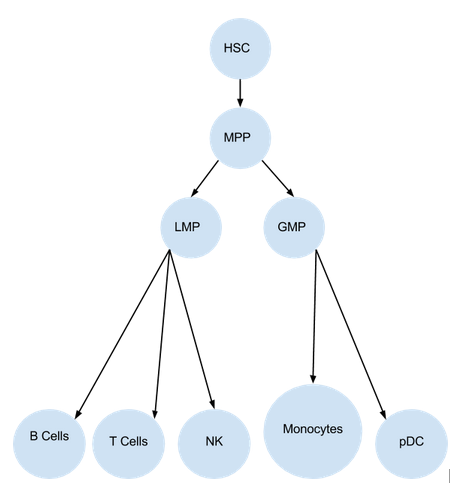
\includegraphics[width=120mm]{cell_types_flow_chart.jpg}
    \caption{Cell progression}
\end{figure}


 The flowchart below shows how the different cell types evolve. The HSC are the first type of cells which divide and form the MPP cells. The MPP cells further divide and form LMP cells as well as GMP cells. The GMP cells further evolve into pDC and Monocytes, whereas the LMPs evolve produce B-cells, T-cells and NK type cells.  


\section{Machine Learning Techniques and Application}
\label{MLalgorithms}


Our dataset contains a huge dataset of various cells and a metric for how much a given protein is represented in that cell. Specifically the data matrix has dimension {$ n \times p $} where {$n = $} number of cells considered and {$ p = $} number of proteins for which have a number representing the amount of protein expression in the cell. The initial dataset is in {$ \mathbb{R}^p $}. In order to reduce this to some {$\mathbb{R}^k$} (e.g. {$\mathbb{R}^2 $} or {$\mathbb{R}^3$}), we use various linear and non-linear techniques to best map the distances of points in a higher dimensional space {$\mathbb{R}^p$} to a lower dimension {$\mathbb{R}^k$} we can visualize.

\subsection{Linear Methods}
\subsubsection{Principal Component Analysis (PCA)}
Principal component analysis allows us to find {$k$} principal components in order of decreasing influence of samples to the overall mean. In order to run this algorithm, we consider {$ \{x^{(i)}; i=1,\ldots,m\} $} where {$ \{1,\ldots,m\} \in \mathbb{R}^p$} where the set of {$m$} proteins is some subset of the protein set {$p$}  that are most representative in detecting cancerous cells (in our case 41 proteins). In particular each {$x_j^{(i)}$} is a measure of how much the protein {$ i $} is represented in cell {$j$}. Since we cannot visualize this data of {$ j $} cells in {$ \mathbb{R}^m $} we use PCA to preserve the variance by converting these {$x^{(i)}$}'s into principal components (i.e. new unitless axes that contain most of the information within just a first few principal components).

Before we apply the algorithm, however, we need to preprocess the data by subtracting the mean and normalizing the values. The mean centering is key to ensure the first principal component doesn't just represent the mean and the normalizing ensures each protein is weighted equally in the algorithm (going forward we may want to weight them as some proteins may be more relevant in determining certain cell types). 

Finally, we apply PCA, which maximizes the variance of projections {$\frac{1}{m}\sum_{i=1}^m(x^{(i),T}u)^2$} by finding the eigenvectors of the covariance matrix {$\frac{1}{m}\sum_{i=1}^m x^{(i)}x^{(i),T}$} and finds the {$ k $} eigenvectors {$ u_1,\ldots,u_k $} which then define the new axes (i.e. the principal components) where:
\begin{center}
{$ y^{(i)} = \left[ {\begin{array}{cc}
   u_1^Tx^{(i)}  \\
   \vdots  \\
   u_1^Tx^{(i)}
  \end{array} } \right] = PC^{(i)} $}
\end{center}

\subsubsection{Classical Multidimensional Scaling (CMDS)}
Similar to PCA, MDS aims to replot each data point in a reduced dimension. As above, assume we want to reduce points in {$\mathbb{R}^m$} to {$ \mathbb{R}^k $}. Specifically we are considering {$k=2$} and {$k=3$}. MDS then outputs an embedding of points {$x_1,\ldots,x_j \in \mathbb{R}^k $} where {$j$} is the number of cells (i.e. number of samples). 

For any two of the {$j$} given cells {$ x_a $} and {$x_b$} in the original space {$\mathbb{R}^m$}we define a distance {$\delta_{a,b} $} between the two points in the higher dimension. In classical CMDS, this is just the Euclidean distance between the points (e.g. {$\sqrt{(x_{a,1}-x_{b,1})^2 + (x_{a,2}-x_{b,2})^2}$} for {$\mathbb{R}^2$}). Thus the constraint on the embedding of points {$x_1,\ldots,x_j \in \mathbb{R}^k $} is that {$ || x_a -x_b||\approx \delta_{a,b} $}. In other words we want to solve the optimization problem with the constraint: 
\begin{center}
{$ \min\limits_{x1,\ldots,x_j} \sum_{a<b} (|| x_a -x_b|| - \delta_{a,b})^2 $}
\end{center}

\subsubsection{Stochastic Neighbor Embedding (SNE)}
This is the first non-linear method we will try, however, unlike other non-linear methods, SNE, as suggested by the name, is a probabilistic approach that aims to preserve the distribution of neighbor identities. SNE, rather than just matching Euclidean distances,  SNE searches for a set of {$ k $} lower-dimensional vectors who's probability distributions best match the probability distributions over all potential neighbors of points in the higher dimension. [1]

More specifically, if we consider all examples {$ x_1,\ldots,x_j \in \mathbb{R}^D $} where {$ D $} is the dimension of each of the rows (i.e. how many proteins for which we have metrics) and similar to PCA we consider a set of {$ y_1,\ldots, y_j \in \mathbb{R}^k $} where {$ k $} is the reduced dimension of proteins, SNE iteratively finds the value of {$ y_1,\ldots,y_j $} that minimizes the difference in probability distribution of neighbors 

\begin{steps}
	\step First select neighbors using either {$ k $} nearest neighbors or by {$ \epsilon $} neighbors. 
	\step Compute the pairwise probability that some {$x_a$} would pick {$ x_b $} as it's neighbor:\\
	\begin{center}
	{$ p_{ab} = \frac{\exp(-d_{ab}^2)}{\sum_{c\neq a}\exp(-d_{ac}^2)} $} 
	\end{center}
	where we define {$ d_{ab} $} to be the dissimilarity between two points in the higher dimension: {$ d_{ab} = \frac{||x_a-x_b||^2}{2\sigma_i^2} $} where {$ \sigma_i^2 $} is the variance of the Gaussian distribution (i.e. the width of the Gaussian kernel. 
	
	Likewise, we can calculate the same probabilities for each pairwise point in the lower dimensional space. (Note: the distributions have a fixed variance): 
	\begin{center}
		{$ q_{ab} = \frac{\exp(-||y_a-y_b||^2)}{\sum_{c\neq a} \exp(-||y_a-y_c||^2)} $}
	\end{center}
	\step Compute a cost function that represents the difference between {$ p_{ab} $} and {$ q_{ab} $} (Kullback-Leibler divergence) and that can be minimized:
	\begin{center}
		{$ J = \sum_a\sum_b p_{ab} \log\frac{p_{ab}}{q_{ab}} $}
	\end{center}
	\step Finally, in order to find the set of {$ y_1,\ldots,y_j \in \mathbb{R}^k $} we iteratively use steepest descent which will eventually converge (given that the function is convex). We use an arbitrary variable {$ c $} to describe each step in the descent algorithm:
	\begin{center}
		{$ y^{(c+1)} = y^{(c)} - \eta^{(c)}\nabla J^{(c)}  $}
	\end{center}
	where {$ \eta^{(c)} $} is the learning rate and the gradient {$ \nabla J^{(c)} $} is: 
	\begin{center}
		{$  \nabla J = \big[ \big(\frac{\partial J}{\partial y_1}\big)^T, \ldots ,\frac{\partial J}{\partial y_j}\big)^T\big]^T  $}\\
		{$ \frac{\partial J}{\partial y_a} = 2\sum_b (y_a - y_b)(p_{ab}-q_{ab}+p_{ba} - q_{ba}) $}
	\end{center}
	The naive SNE has a fairly slow convergence time, therefore there are multiple variations on this algorithm [1]. 
\end{steps}

We have left room to also try out t-SNE and vi-SNE which are specialized methods that have been proven to work on similar sets of cell data. 	
\subsubsubsection{t-SNE}


\subsubsubsection{vi-SNE}


\section{Current Results}

Below we present a PCA analysis of the Basal data. Since surface proteins are more standard proteins for cell type identification, we compare PCA run on surface protein data to PCA run on all protein data. Additionally, we show PCA for all cell types as well as PCA for individual subsets of cells (i.e. B Cells, TCells, Monocytes, and Stem Cells).

In particular we compare a classification for all proteins and just the surface proteins for each of the cell types. That is, Figure 2 and Figure 3 are displaying the same thing except 2 displays it for all proteins (surface + intracellular) and 3 for just the surface proteins. 

\begin{figure}[htp]
\centering
  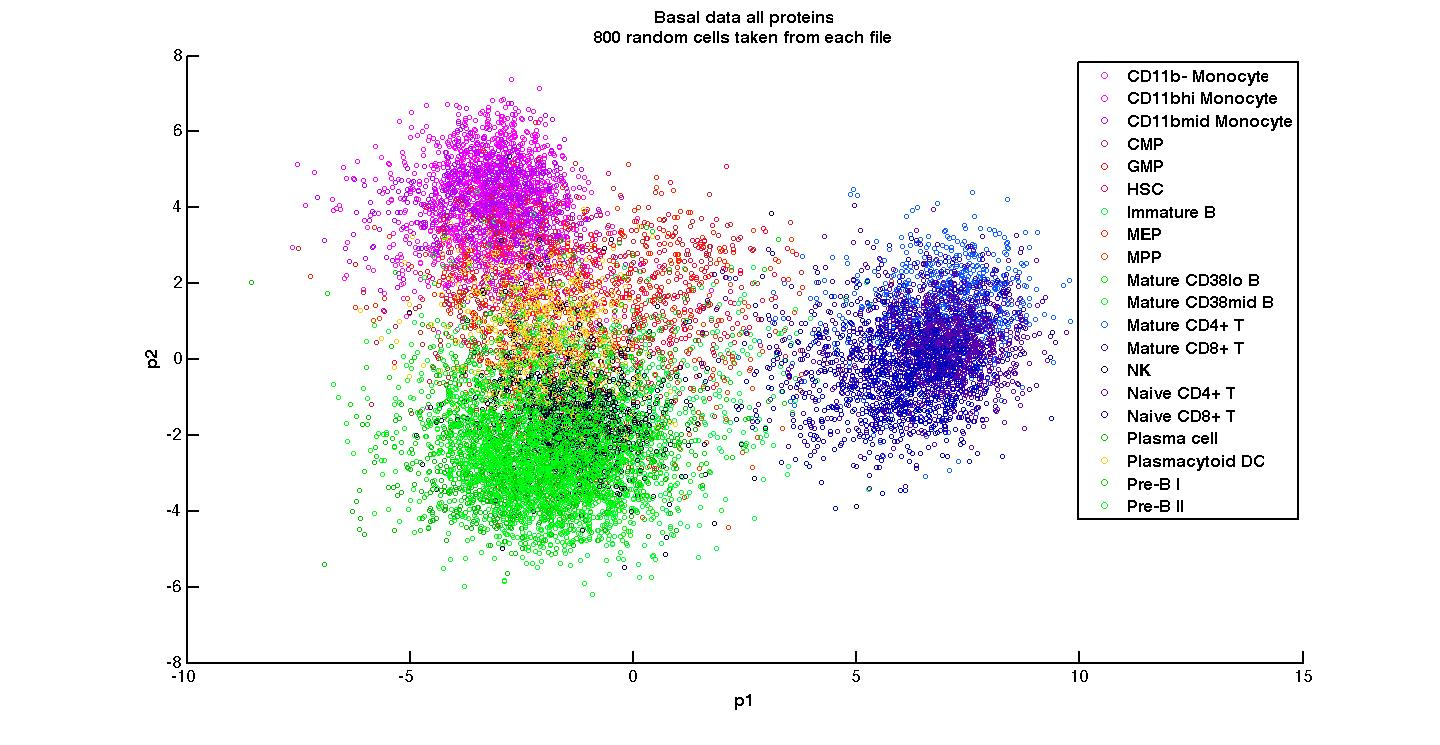
\includegraphics[width=120mm]{Basal_AllProtein_AllCells.jpg}
  \caption{Basal, all proteins, all cell types}
\end{figure}

\begin{figure}[htp]
  \centering
  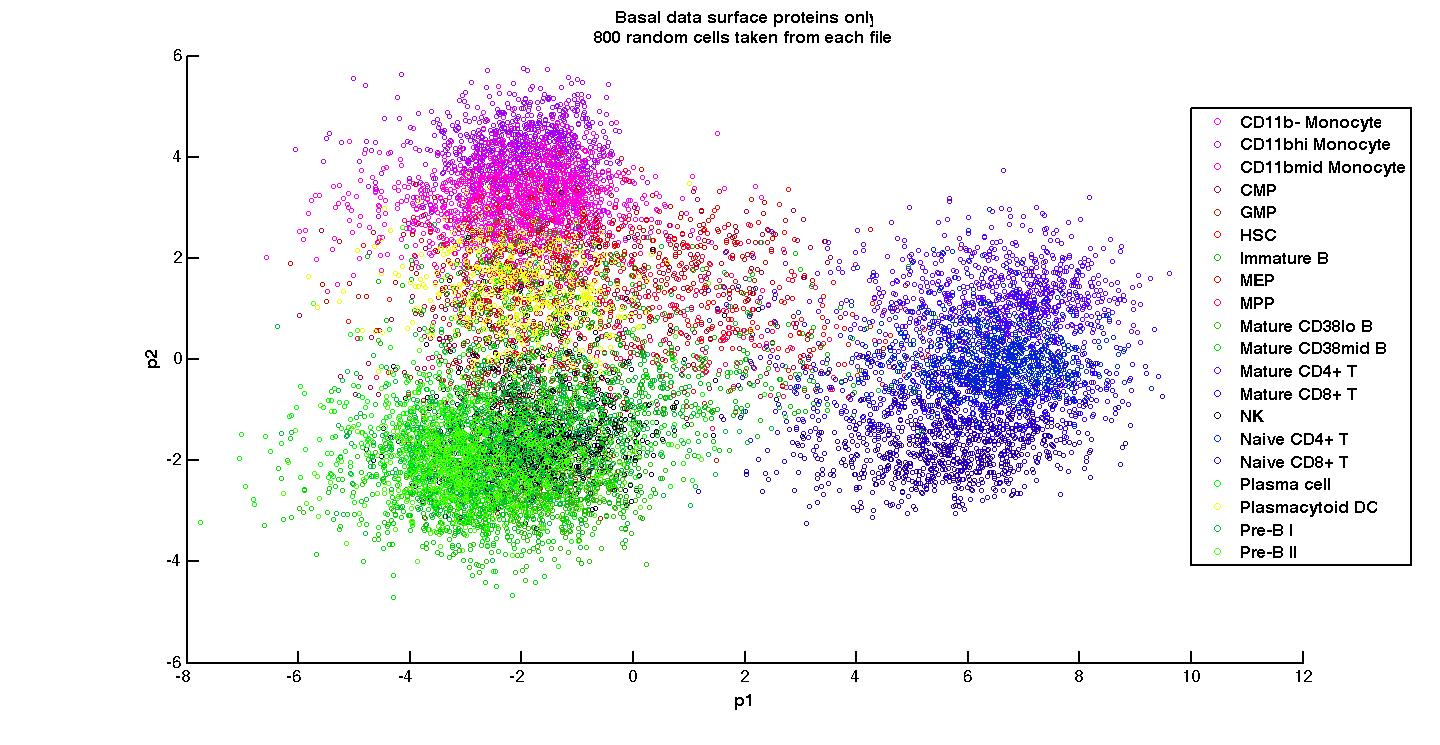
\includegraphics[width=120mm]{Basal_SurfaceProtein_AllCells.jpg}
  \caption{Basal, surface proteins, all cell types}
\end{figure}

\begin{figure}
 \centering
 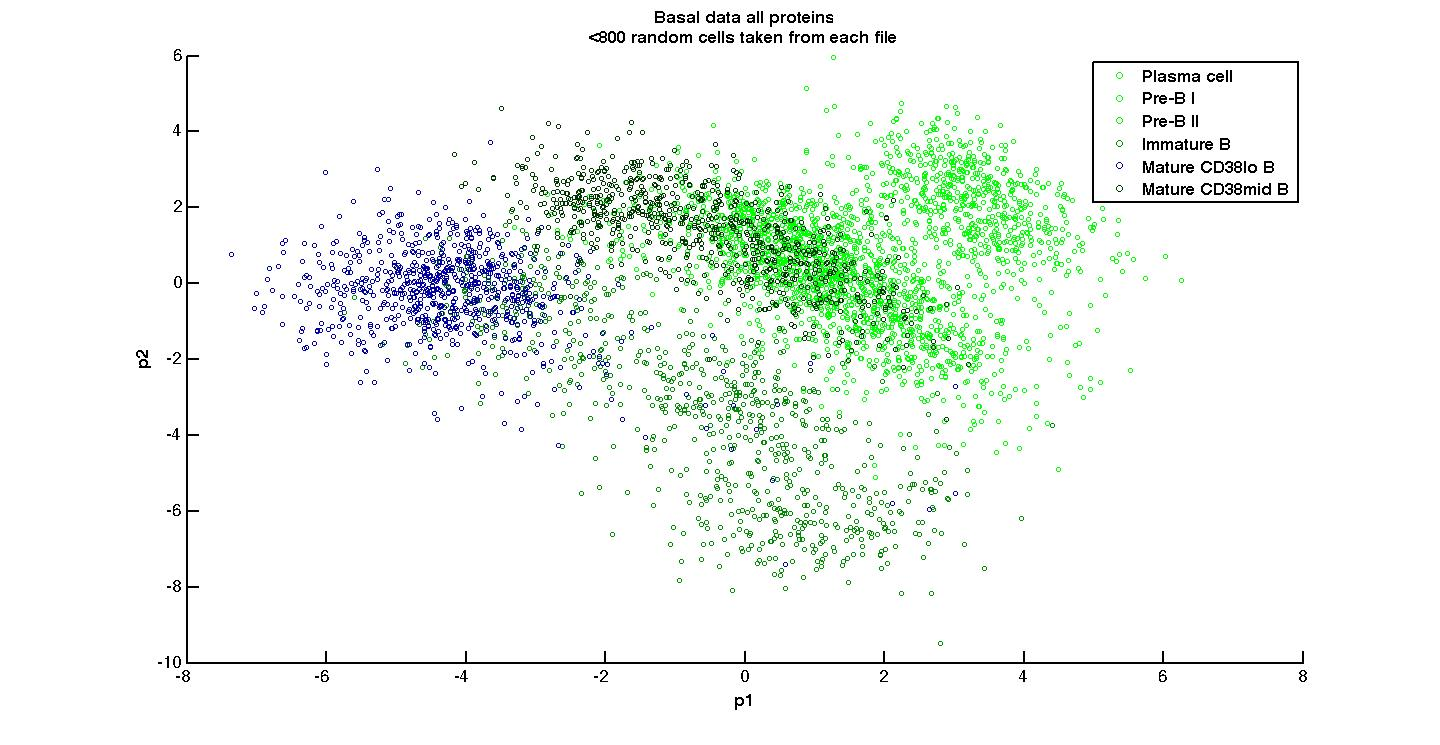
\includegraphics[width=120mm]{Basal_AllProtein_BCells.jpg}
 \caption{Basal, all proteins, B cells}
\end{figure}

\begin{figure}
 \centering
 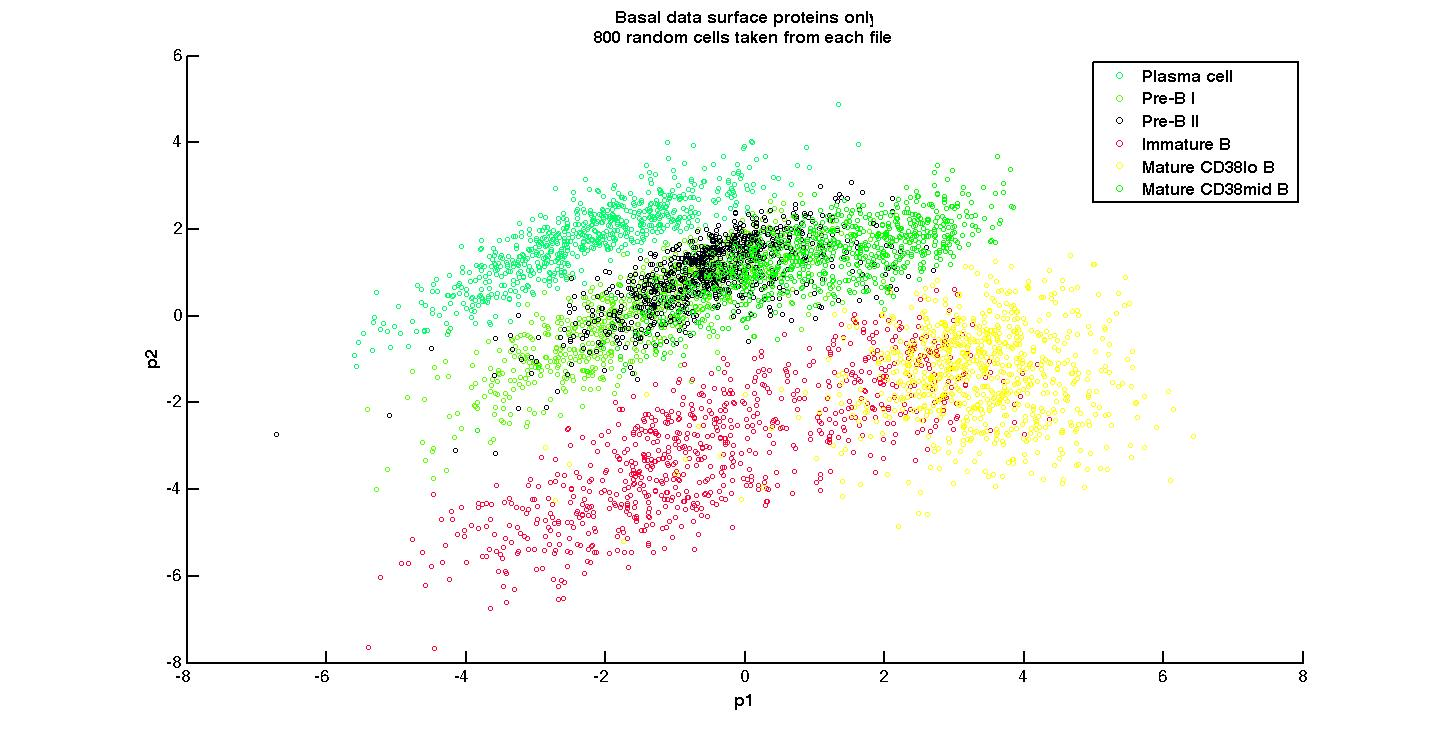
\includegraphics[width=120mm]{Basal_SurfaceProtein_BCells.jpg}
 \caption{Basal, surface proteins, B cells}
\end{figure}

\begin{figure}
  \centering
    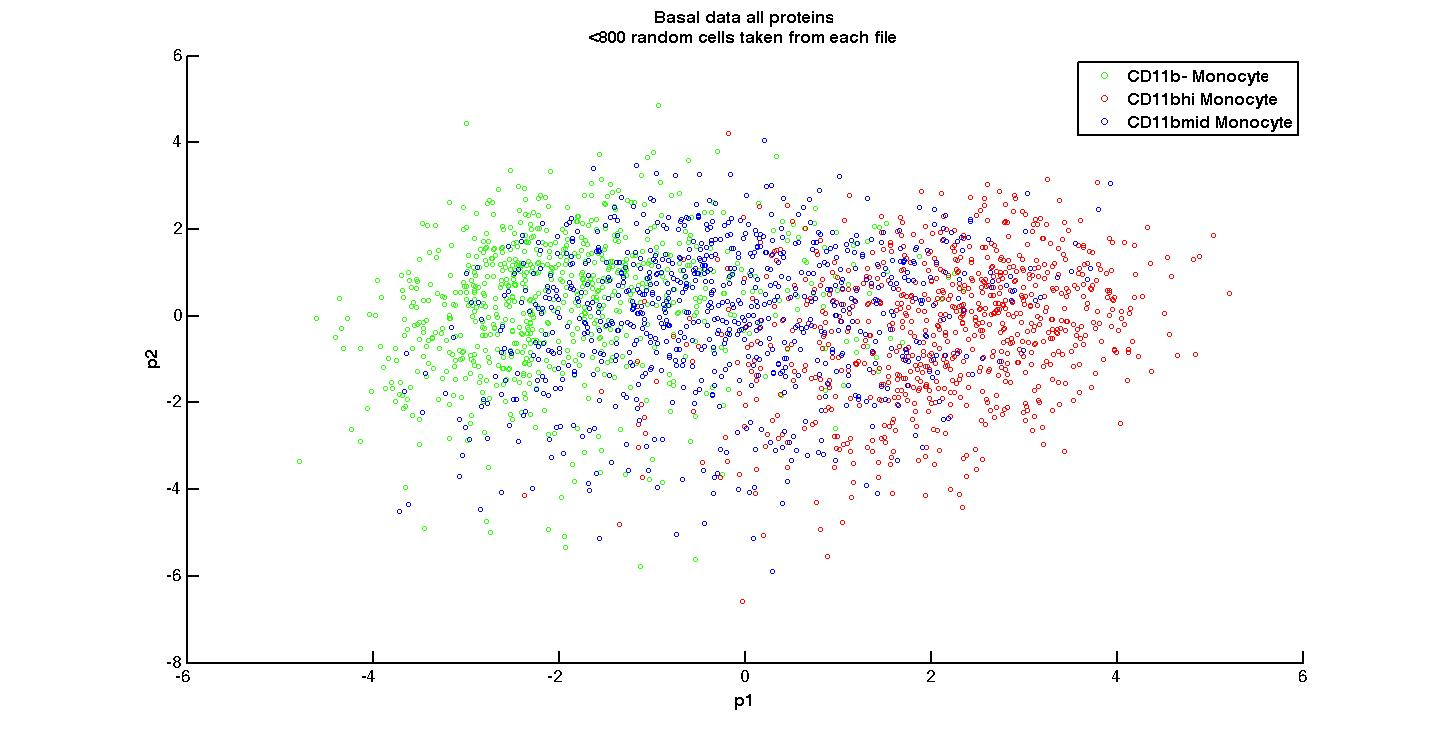
\includegraphics[width=120mm]{Basal_AllProtein_Monocytes.jpg}
     \caption{Basal, all proteins, monocytes}
\end{figure}

\begin{figure}
  \centering
    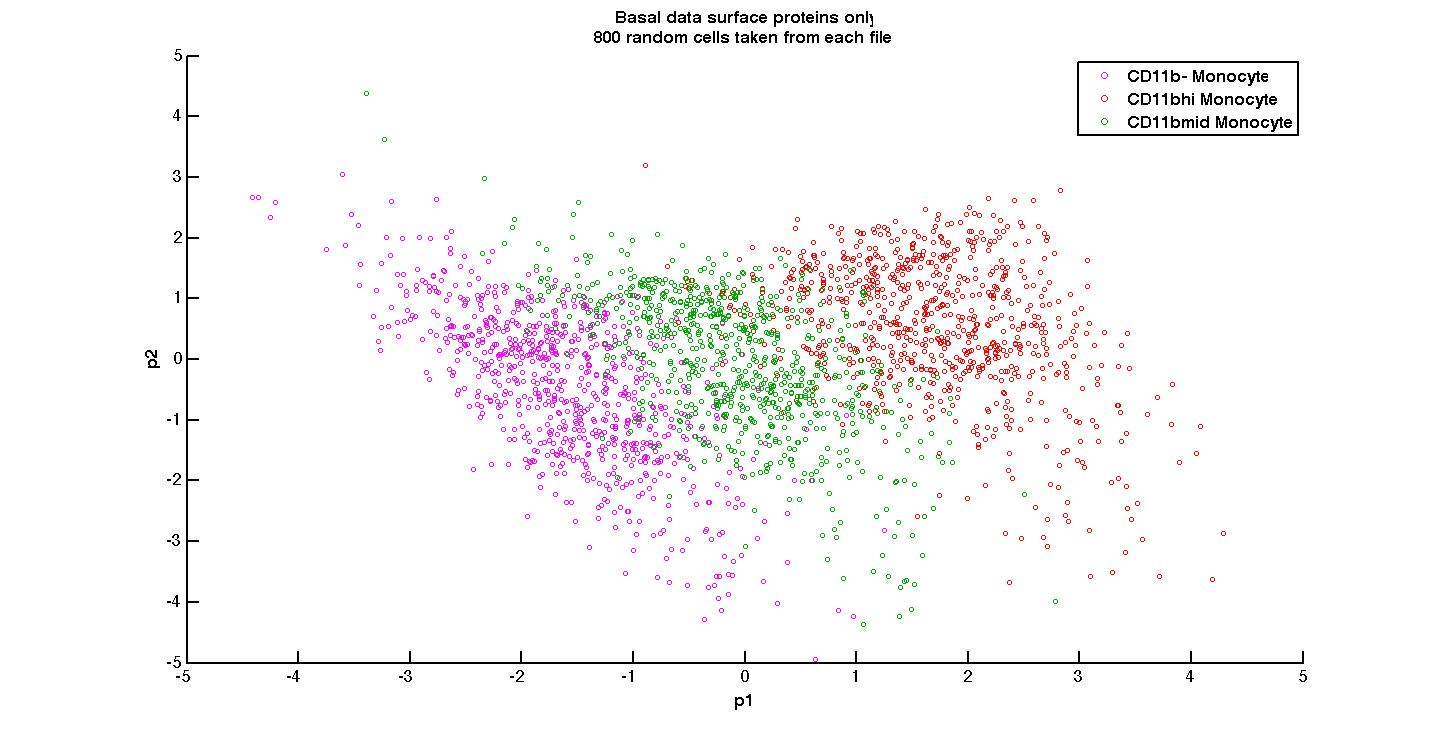
\includegraphics[width=120mm]{Basal_SurfaceProtein_Monocytes.jpg}
     \caption{Basal, surface proteins, monocytes}
\end{figure}

\begin{figure}
 \centering
    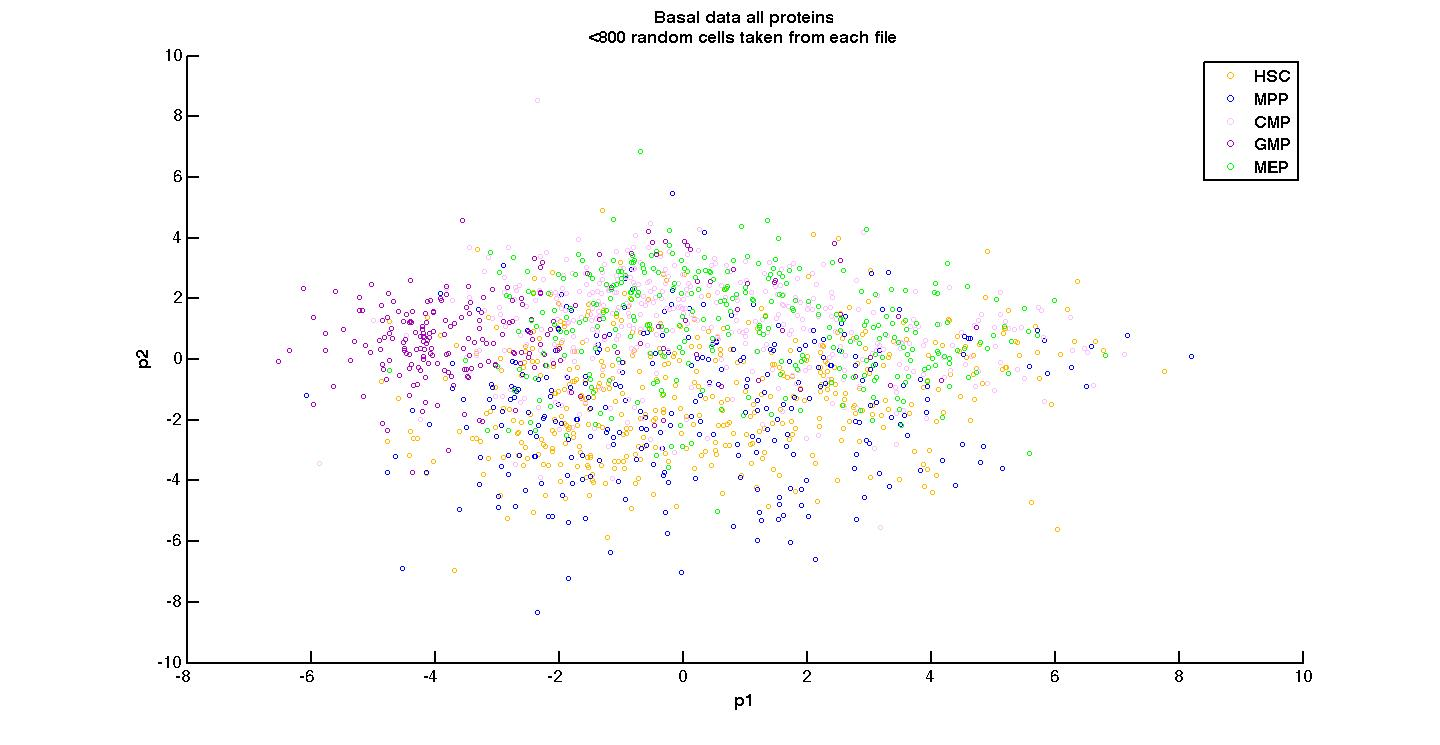
\includegraphics[width=120mm]{Basal_AllProtein_StemCells.jpg}
    \caption{Basal, all proteins, stem cells}
\end{figure}

\begin{figure}
 \centering
    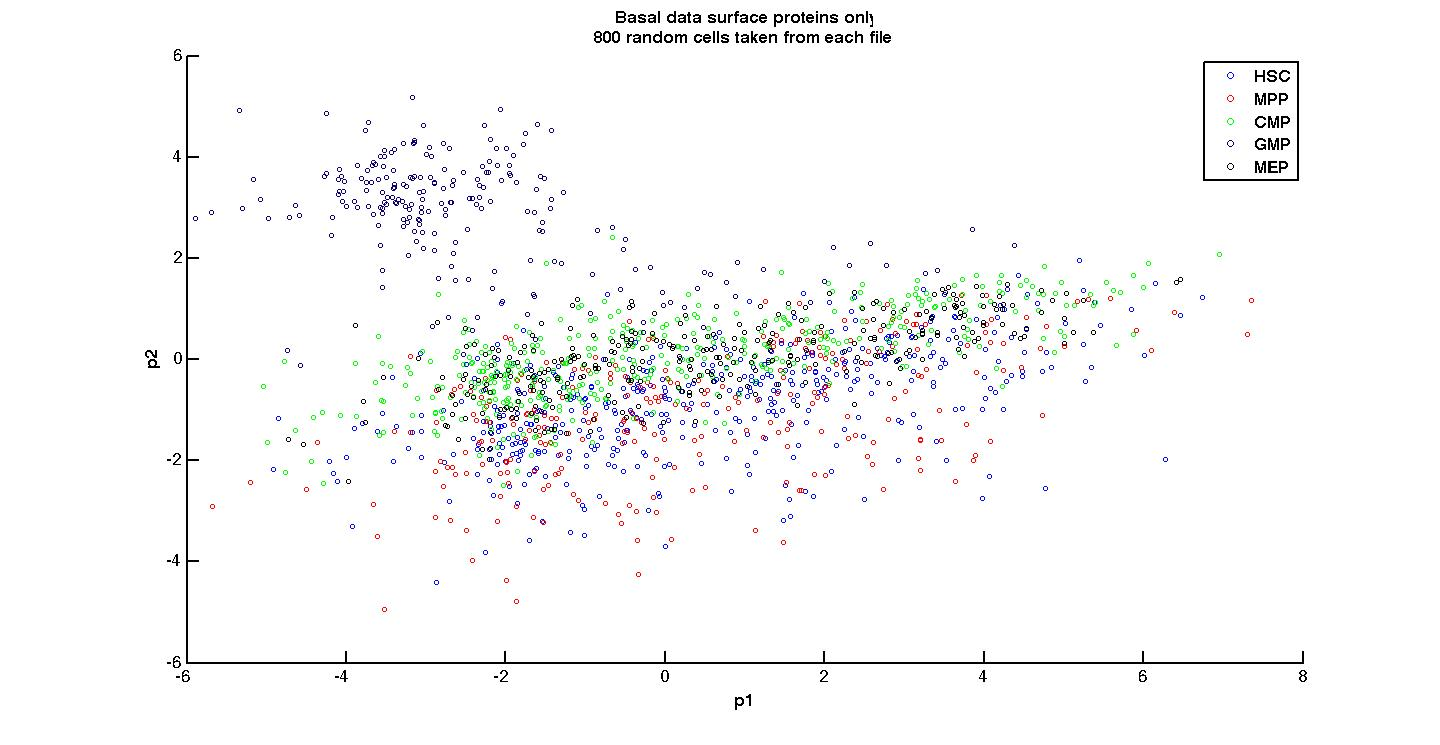
\includegraphics[width=120mm]{Basal_SurfaceProtein_StemCells.jpg}
    \caption{Basal, surface proteins, stem cells}
\end{figure}

\begin{figure}
 \centering
    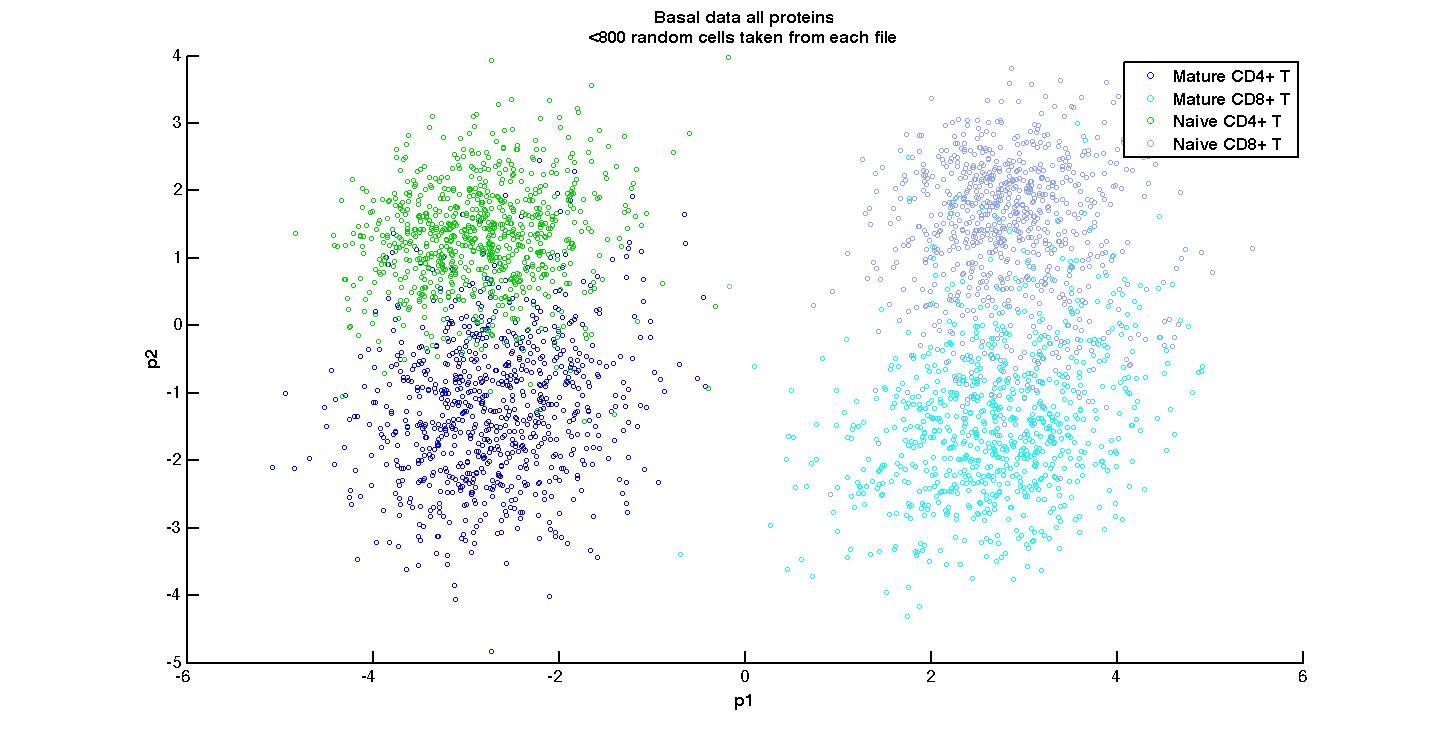
\includegraphics[width=120mm]{Basal_AllProtein_TCells.jpg}
    \caption{Basal, all proteins, T cells}
\end{figure}

\section{Conclusion / Looking Ahead (End of Project Goals)}
Currently we have observed dimensional reduction using PCA and have compared various plots to determine qualitatively how well we can differentiate between the various cells. Specifically, we have been given labelled cell data that characterizes each cell type (and sub-cell type) by its protein characteristics. Our job is to take this labelled data and ensure that we can differentiate between each cluster. That way, once we remove the labels we can run the same trained algorithm on cancer cell data to establish whether a cell is anomalous (i.e. doesn't fit within a cluster) or whether it is �normal�. 

To ensure good classification we have two jobs ahead of us: \\
\begin{itemize}
\item determining a quantitative measure that characterizes how well our algorithm differentiates cells 
\item using that metric to compare other linear and non-linear algorithms (e.g. MDS, SNE, t-SNE, etc). 
\end{itemize}
In doing so, we will run a similar analysis as above where we vary the number of cells and the number of proteins sampled to determine an optimum algorithm and parameter set. 

Finally, we will use the data to try and map out the life cycle of a cell. Although our data is not temporal and cannot be sampled in-situ, we plan to use a community of cells and sample a different cell within the same community at different stages of their life to determine if we can create a volume in 3D space that subtends the life cycle of a healthy cell. With this we can determine whether a cancer cell is anomalous regardless of which part of the lifecycle it may be currently in. 

\section*{Acknowledgments}

We would like to thank Karen Sachs and Andrew Gentles for providing the data and guidance for the project. 

\section*{References}

\small{
[1]\url{http://www.postech.ac.kr/~seungjin/publications/ijcnn04_kjnam.pdf}

[2]\url{http://www.nature.com/nbt/journal/v31/n6/full/nbt.2594.html#introduction}

[3]\url{http://jmlr.org/papers/volume9/vandermaaten08a/vandermaaten08a.pdf}

[3] Hasselmo, M.E., Schnell, E. \& Barkai, E. (1995) Dynamics of learning
and recall at excitatory recurrent synapses and cholinergic modulation
in rat hippocampal region CA3. {\it Journal of Neuroscience}
{\bf 15}(7):5249-5262.
}

\end{document}
